\documentclass[tikz,border=3pt]{standalone}
\usepackage{amsmath}
\usepackage{tikz}
\usetikzlibrary{shapes.geometric,arrows.meta,patterns,calc}

\begin{document}
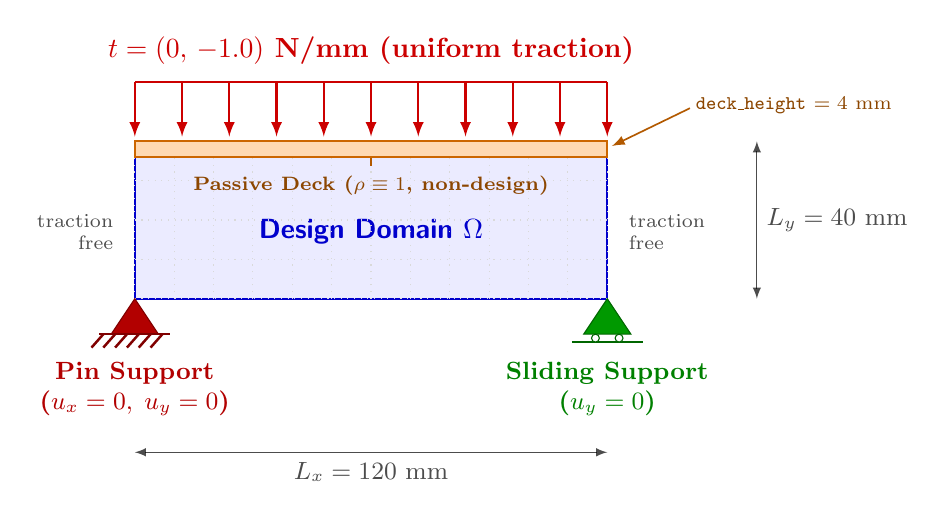
\begin{tikzpicture}[scale=1.0, >=latex]
  % SimplySupportedBridge2d: 120 x 40 mm, 绘图比例 0.05 -> 6.0 x 2.0
  % Design Domain
  \draw[thick, fill=blue!8, draw=blue!80!black] (0,0) rectangle (6,2);
  \node[font=\bfseries\sffamily, color=blue!80!black] at (3,0.85) {Design Domain $\Omega$};

  % Grid overlay
  \draw[step=0.5, gray!30, dotted] (0,0) grid (6,2);

  % Passive deck strip (top band of thickness deck_height = 4 mm -> 0.2)
  \fill[orange!30] (0,1.8) rectangle (6,2);
  \draw[thick, orange!80!black] (0,1.8) rectangle (6,2);
  \draw[orange!70!black] (3,1.79) -- (3,1.68);
  \node[below, font=\scriptsize\bfseries, color=orange!55!black] at (3,1.68)
    {Passive Deck ($\rho \equiv 1$, non-design)};

  % Uniform distributed traction on the whole Top Edge (y = 40)
  \draw[thick, red!80!black] (0, 2.75) -- (6, 2.75);
  \foreach \x in {0.0, 0.6, 1.2, 1.8, 2.4, 3.0, 3.6, 4.2, 4.8, 5.4, 6.0} {
    \draw[->, thick, red!80!black] (\x, 2.75) -- (\x, 2.06);
  }
  \node[above, red!80!black, font=\bfseries] at (3, 2.85)
    {$t = (0,\,-1.0)\text{ N/mm}$ (uniform traction)};

  % Pin Support at Bottom Left (0, 0): u_x = u_y = 0
  \draw[fill=red!70!black, draw=red!50!black] (0,0) -- (-0.3,-0.45) -- (0.3,-0.45) -- cycle;
  \draw[thick, red!50!black] (-0.45,-0.45) -- (0.45,-0.45);
  \foreach \i in {-0.4,-0.25,-0.1,0.05,0.2,0.35} {
    \draw[line width=0.9pt, red!50!black] (\i,-0.45) -- (\i-0.15,-0.62);
  }
  \node[below, red!70!black, font=\small\bfseries, align=center] at (0,-0.68)
    {Pin Support\\($u_x = 0,\; u_y = 0$)};

  % Sliding (roller) Support at Bottom Right (120, 0): u_y = 0
  \draw[fill=green!60!black, draw=green!40!black] (6,0) -- (5.7,-0.45) -- (6.3,-0.45) -- cycle;
  \draw[thick, green!40!black] (5.55,-0.55) -- (6.45,-0.55);
  \draw[fill=white, draw=green!40!black] (5.85,-0.5) circle (0.05);
  \draw[fill=white, draw=green!40!black] (6.15,-0.5) circle (0.05);
  \node[below, green!50!black, font=\small\bfseries, align=center] at (6,-0.68)
    {Sliding Support\\($u_y = 0$)};

  % Traction-free sides
  \node[left, gray!60!black, font=\scriptsize, align=right] at (-0.15,0.85) {traction\\free};
  \node[right, gray!60!black, font=\scriptsize, align=left] at (6.15,0.85) {traction\\free};

  % deck_height 引注 (强调它只有域高的 1/10, 直接标尺寸线会看不清)
  \draw[->, orange!70!black, semithick] (7.05,2.42) -- (6.06,1.94);
  \node[right, font=\scriptsize, color=orange!55!black] at (7.0,2.45)
    {\texttt{deck\_height} $= 4\text{ mm}$};

  % Dimensions
  \draw[<->, opacity=0.7] (0,-1.95) -- (6,-1.95) node[midway, below, font=\small] {$L_x = 120\text{ mm}$};
  \draw[<->, opacity=0.7] (7.9,0) -- (7.9,2) node[midway, right, font=\small] {$L_y = 40\text{ mm}$};
\end{tikzpicture}
\end{document}
